\begin{frame}
\frametitle{Aufgabe 1b}
\framesubtitle{}
    \begin{itemize}
        \item Der Einschaltevorgang der Geräte am Messaufbau kann die Messung
    beeinflussen.
        \item Untersuchung des Einflusses auf eine Gleichstrommessung
    \end{itemize}
\end{frame}
\begin{frame}
\frametitle{Aufgabe 1b}
\framesubtitle{1: Messungen}
\begin{figure}[H]
\begin{center}
    \fbox{
        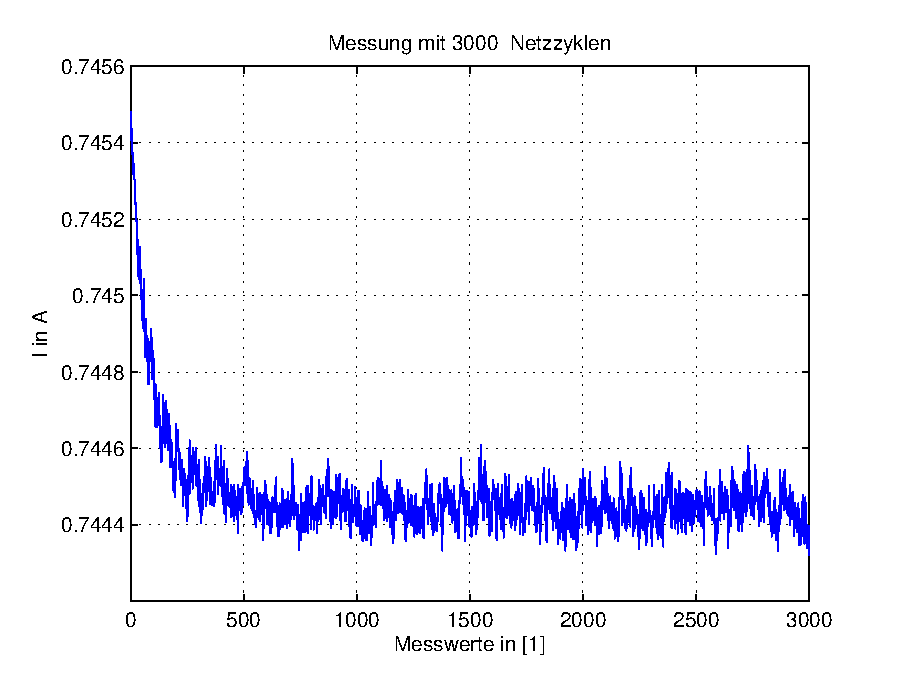
\includegraphics[scale=0.60]{./img/1b13000.eps}
    }
    \caption{Graph 1}
\end{center}
\end{figure}
\end{frame}

\begin{frame}
\frametitle{Aufgabe 1b}
\framesubtitle{1: Messungen}
\begin{figure}[H]
\begin{center}
    \fbox{
        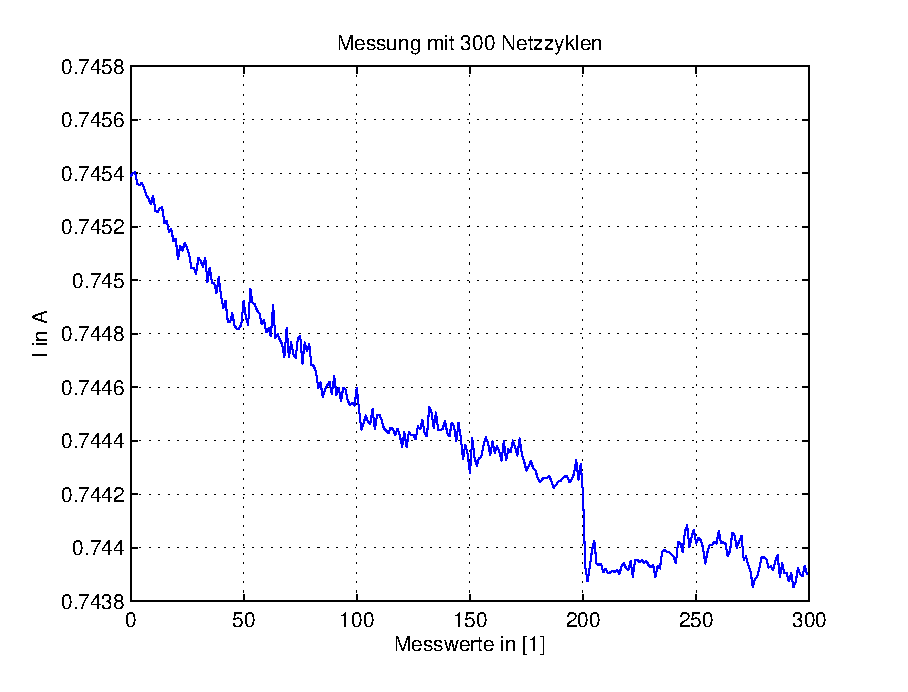
\includegraphics[scale=0.60]{./img/1b1300.eps}
    }
    \caption{Graph 2}
\end{center}
\end{figure}
\end{frame}
\begin{frame}
\frametitle{Aufgabe 1b}
\framesubtitle{Ergebnis}
    Man betrachtet:
    \begin{itemize}
        \item Starker Abfall der Stromstärke von $0-200$
        \item Annährung and den Endwert von $200-500$ in Graph $1$
        \item Sprung auf den Endwert bei $200$ in Graph $2$
    \end{itemize}
    Mögliche Erklärung:
     \begin{itemize}
         \item Bauteile des Geräts müssen sich erst aufwärmen oder einschwingen
         \item Bestimmte Bauteile funktionieren erst ab einer bestimmten
         Temperatur (Sprung in Graph $2$)
     \end{itemize}
    Sofortige Messung nach Einschalten des Geräts liefert keine verlässlichen
    Werte! \\
    Empfehlung des Herstellers: Gerät $30$ Minuten warmlaufen lassen
\end{frame}
\begin{frame}
\frametitle{Aufgabe 1b}
\begin{itemize}
    \item Die Wahl der Integrationszeit kann die Messung beeinflussen.
    \item Der Einfluss der Integrationszeit wurde durch verschiedene
    Netzzyklenzahlen und freie Zeiteinstellung getestet.
\end{itemize}
\end{frame}
\begin{frame}
\frametitle{Aufgabe 1b}
\framesubtitle{2:Messungen}
\begin{tabular}{c|c c c c}
    NPLC   & Maximum    & Minimum    & Mittelwert  &Standardabweichung \\
    \hline
    0,006  & 0,201529   & 0,19882    & 0,20011369  &5,69E-04\\
    0,02   & 0,201495   & 0,198794   & 0,200125373 &5,95E-04\\
    0,06   & 0,201637   & 0,198639   & 0,20012612  &7,70E-04\\
    0,2    & 0,201453   & 0,198895   & 0,200099427 &6,00E-04\\
    1      & 0,200122   & 0,200035   & 0,200076633 &1,54E-05\\
    10     & 0,20006    & 0,199953   & 0,199991067 &2,57E-05
\end{tabular}
\end{frame}
\begin{frame}
\frametitle{Aufgabe 1b}
\framesubtitle{2: Ergebnis}
     Je größer die Standardabweichung, desto mehr liegen Minima und Maxima
     voneinander entfernt $\rightarrow$ mehr Rauschen
     \begin{itemize}
         \item Größte Standardabweichung bei $0.6$ NPLC
         \item Kleinste Standardabweichung bei $10$ NPLC
     \end{itemize}
     $\rightarrow$ Beim Mitteln über Teilzyklen hebt sich das Rauschen nicht
     auf \\
     $\rightarrow$ Beim Mitteln über ganzzahlige Netzzyklen wird das Rauschen
     herausgefiltert \\
     $\rightarrow$ Erhöhung der ganzzahligen Netzzyklen verbessert die
     Genauigkeit
\end{frame}
\begin{frame}
\frametitle{Aufabe 1b}
\framesubtitle{3:Messungen}
\begin{tabular}{c|c c c c}
    NPLC   & Maximum    & Minimum    & Mittelwert  &Standardabweichung \\
    \hline
    0,006  & 0,201529   & 0,19882    & 0,20011369  &5,69E-04\\
    0,02   & 0,201495   & 0,198794   & 0,200125373 &5,95E-04\\
    0,06   & 0,201637   & 0,198639   & 0,20012612  &7,70E-04\\
    0,2    & 0,201453   & 0,198895   & 0,200099427 &6,00E-04\\
    1      & 0,200122   & 0,200035   & 0,200076633 &1,54E-05\\
    10     & 0,20006    & 0,199953   & 0,199991067 &2,57E-05\\
    \hline
    freie Int.& & & &\\
    \hline
    25 ms  & 0,200182   & 0,199796   & 0,19999138  &1,16E-04
\end{tabular}
\end{frame}
\begin{frame}
\frametitle{Aufgabe 1b}
\framesubtitle{3: Ergebnis} 
    Mitteln über eine frei gewählte Zeit ist ungenauer als vielfache NPLCs. \\
    $\rightarrow$ Netzzyklen werden nicht exakt abgeschlossen, Rauschen wird
    nicht vollständig weggehoben

    Wie soll gemittelt werden?
    \begin{itemize}
        \item Teilzyklen: erhöht Rauschen aber verkürzt Messzeit $\rightarrow$
        nur bei sehr vielen Messreihen
        \item vielfache NPCLs: verringert Rauschen aber längere Messzeit
        \item freie Zeit: Nur wenn freie Integrationszeit notwendig
    \end{itemize}
\end{frame}


